\apendice{Especificación de diseño}

\section{Introducción}
Una vez realizado el estudio y especificación de los requisitos de la aplicación web, se debe realizar el diseño de la misma.\\
En este apartado se pretende aportar información sobre el diseño de los datos que utiliza la aplicación junto al diseño procedimental y arquitectónico del proyecto.

\section{Diseño de datos}
Gracias a la especificación de requisitos y casos de uso, se puede obtener una visión global de la aplicación que permite deducir las entidades, acompañadas de sus datos, necesarias para poder cumplir con lo requerido.\\
En primer lugar, podemos obtener la visión global de las entidades relacionadas mediante el diagrama general de Entidad-Relación de la figura~\ref{DiagramaGeneralE-R}.\\
El diagrama obtenido tiene un gran tamaño y, para mejorar la visualización y comprensión del mismo, se ha decidido dividir en vistas donde se incluyan los datos de cada una de las entidades.\\
La primera vista hace referencia al apartado de mantenimiento académico y se puede ver en la figura~\ref{er_cu1}, la segunda al mantenimiento de profesorado~\ref{er_cu2} y la última a la asignación docente~\ref{er_cu3}.

\figuraApaisadaSinMarco{}{../img/Anexos/Diagrama E-R.pdf}{Diagrama general entidad-relación}{DiagramaGeneralE-R}{}

Del diagrama entidad-relación se puede obtener el diagrama relacional de la figura~\ref{DiagramaRelacional} en el que se pueden ver la tablas que contendrá la base de datos de la aplicación web.

\begin{figure}[!h]
	\centering
	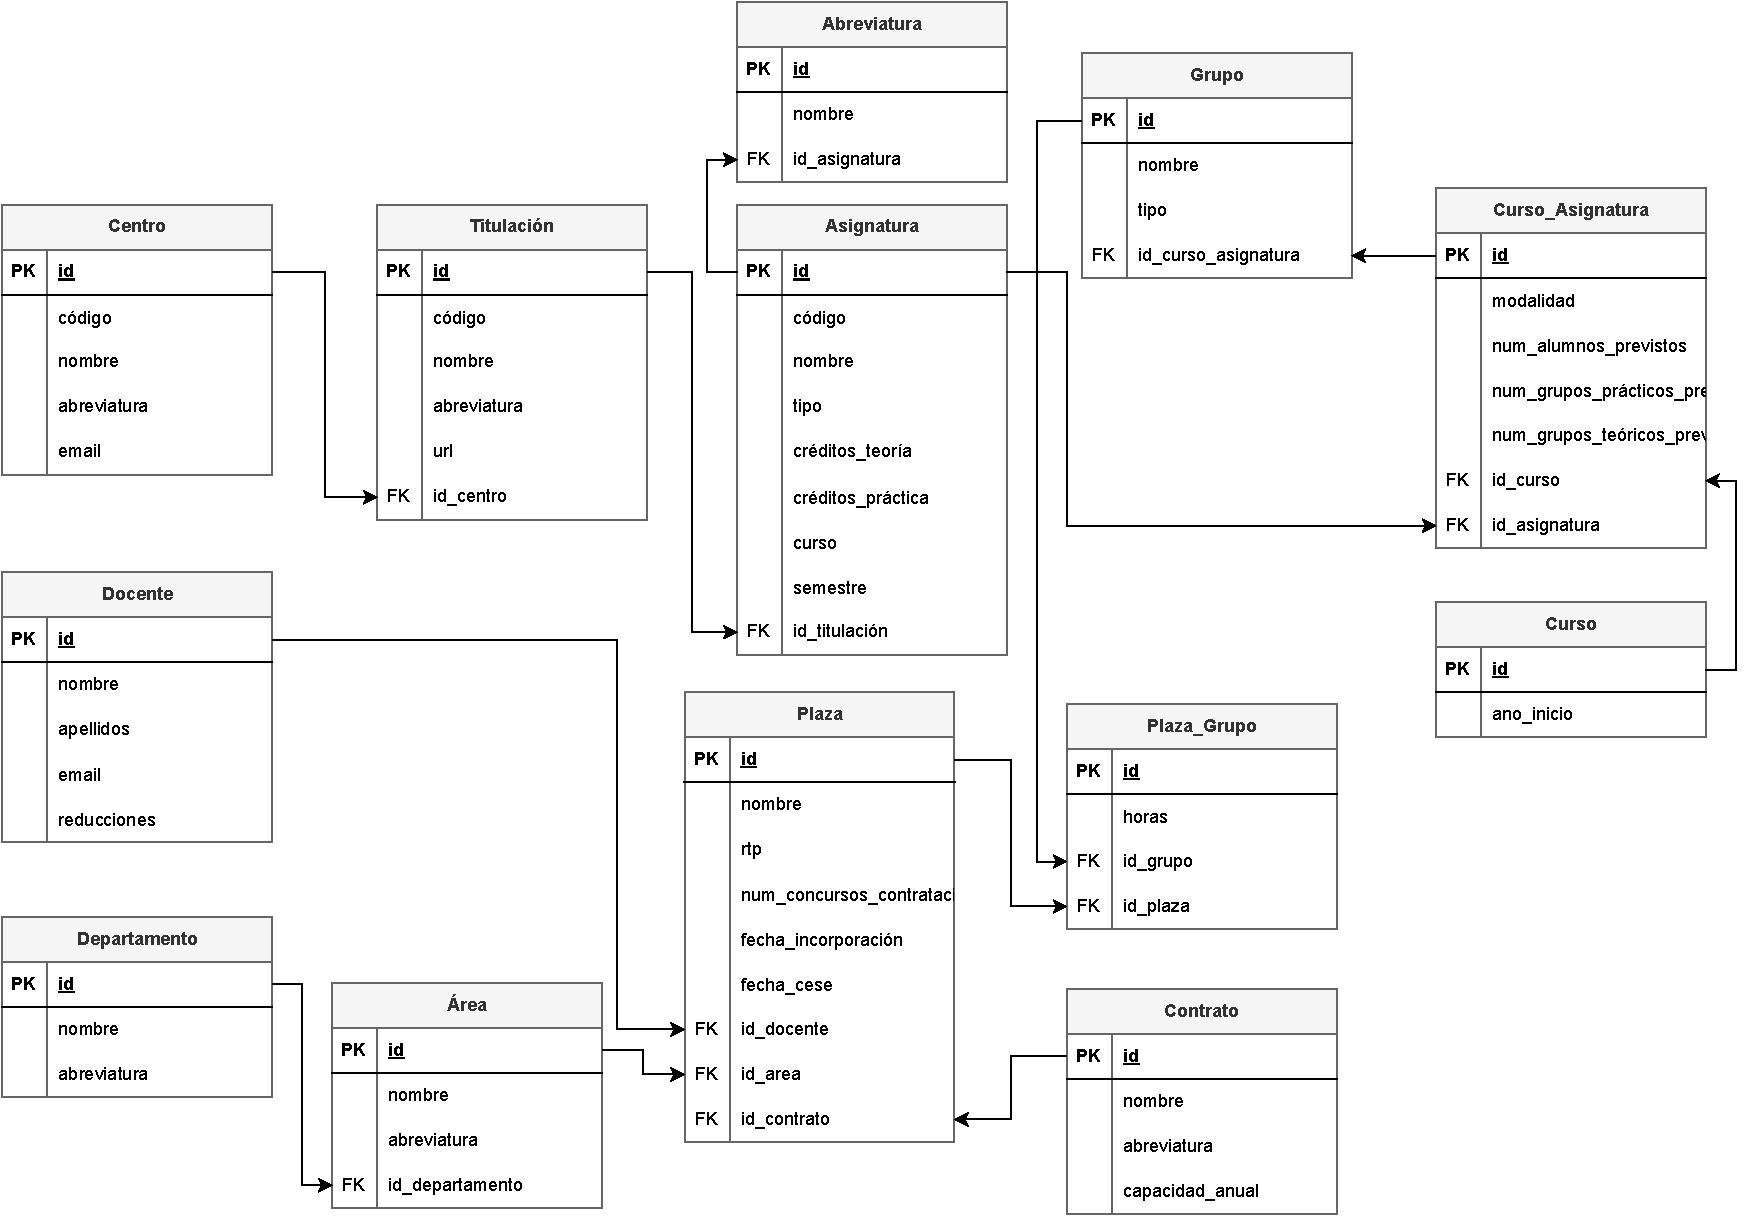
\includegraphics[width=1.2\textwidth]{../img/Anexos/Diagrama relacional.pdf}
	\caption{Diagrama relacional}\label{DiagramaRelacional}
\end{figure}
\section{Diseño procedimental}

\section{Diseño arquitectónico}


